\documentclass[12pt,a5paper]{article}
\usepackage[a4paper, margin=2cm]{geometry}
\usepackage[utf8]{inputenc}
\usepackage{amsmath}
\usepackage{amsfonts}
\usepackage{graphicx}
\usepackage{amssymb}
\usepackage{imakeidx}
\usepackage{listings}
\usepackage{multirow}
\usepackage{hyperref}
\usepackage{cancel}
\usepackage{subfloat}
\usepackage{caption}
\usepackage{multirow}
\usepackage{multicol}
\usepackage{color}
\usepackage{setspace}
\usepackage{subfig}
\usepackage{parskip}
\usepackage[spanish,es-tabla]{babel}
\usepackage{fancyhdr}
\usepackage{schemata}
\usepackage{appendix}
\usepackage{lastpage}
\usepackage{float}

\graphicspath{ {images/parte2-talbot}{images/parte3-fourier}{images/parte4-filtrado}{images/parte5-luz-coherente}{images/talbot-4f} }

%Detalles de la estructura,
\fancyhf{}
\renewcommand{\headrulewidth}{0,5pt}
\thispagestyle{plain}
\pagestyle{fancy}
\fancyhead[L]{Procesado óptico y digital de señales e imágenes}
\fancyhead[R]{Práctica 2}
\fancyfoot[C]{Página \thepage\ de \pageref{LastPage}}



\begin{document}

%Portada
\begin{titlepage}
\centering
\rule{16 cm}{2 pt}
{\scshape\Huge Procesado óptico y digital de señales e imágenes \par}
\vspace{2cm}
{\scshape\Large \textbf{Práctica 2:} Procesado óptico de la información\par}
\rule{16 cm}{2 pt}
\vfill
{\Large \textbf{Alumnos:}\par Alejandro \textcolor{red}{apellidos} \par Adriana \textcolor{red}{apellidos} \par Carlos España Castaño \par}
{\Large Fecha: 16 de noviembre de 2022 \par}
\end{titlepage}



%Índice,
\newpage
\tableofcontents
\newpage



\section{Introducción}





\section{El efecto Talbot}
\textcolor{blue}{Añadir pequeña explicación de la sección}\par
Las distancias a las que se reproduce el campo periódico son ciertas fracciones de la denominada distancia de Talbot, que viene dada por la expresión \ref{ec:zt}:

\begin{center}
    \begin{equation}
        z_T = \frac{2d^2}{\lambda}
        \label{ec:zt}
    \end{equation}
\end{center}


Registramos varias imágenes a distancias en la que se observaba una distribución de intensidad semejante a la del objeto original (franjas transparentes y opacas de igual tamaño), así como a distancias en las que se observaba una distribución de intensidad homogénea:\par

\begin{center}
    \captionof{table}{Distancias fraccionarias de la longitud de Talbot $z_T$}
    \begin{tabular}{|c|c|c|} \hline
        Distancia & Distribución de intensidad & Distancia (fracción de $z_T$)\\ \hline
        18,5 cm & Homogénea & $z_T/4$\\ \hline
        36,8 cm & Franjas claras y oscuras & $z_T/2$\\ \hline
        55,8 cm & Homogénea & $3z_T/4$\\ \hline
        72,9 cm & Franjas claras y oscuras & $z_T$\\ \hline
    \end{tabular}
\end{center}

\textcolor{red}{Hola, aunque en los nombres de los archivos png ponga otros valores, esos eran sólo las lecturas del metro. Las distancias a la cámara son las que aparecen en la tabla.}

A modo de ejemplo, esta es la imagen que se obtuvo a la distancia de Talbot $Z_T$:

\begin{figure}[h!]
    \centering
    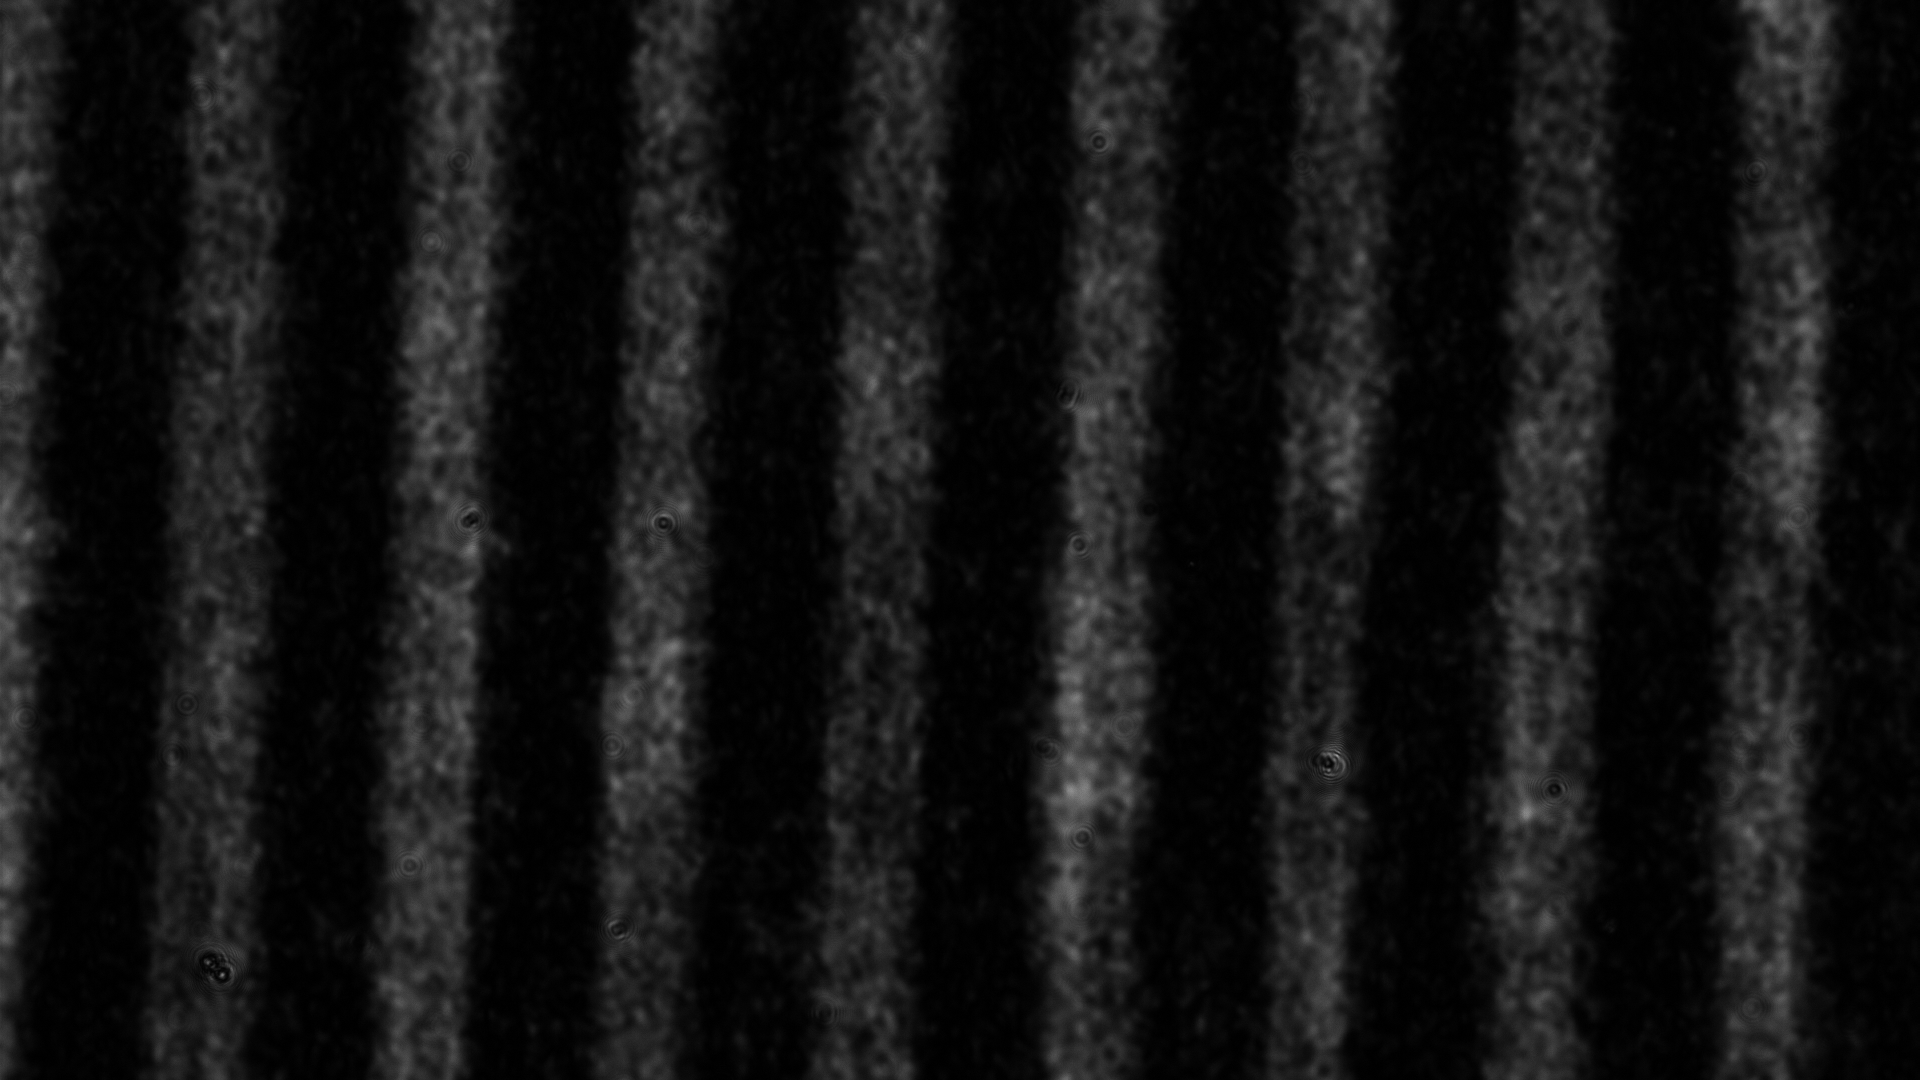
\includegraphics[scale=0.15]{54.8-2a-talbot.png}
    \caption{Imagen del objeto a la distancia de Talbot: $z_T = 72,9 cm$}
    \label{fig:imagen-zt}
\end{figure}

Vemos que se repite el patrón de intensidad del objeto. A una distancia de un cuarto de la distancia de Talbot, $Z_T/4$, esta es la imagen que se obtuvo:

\begin{figure}[h!]
    \centering
    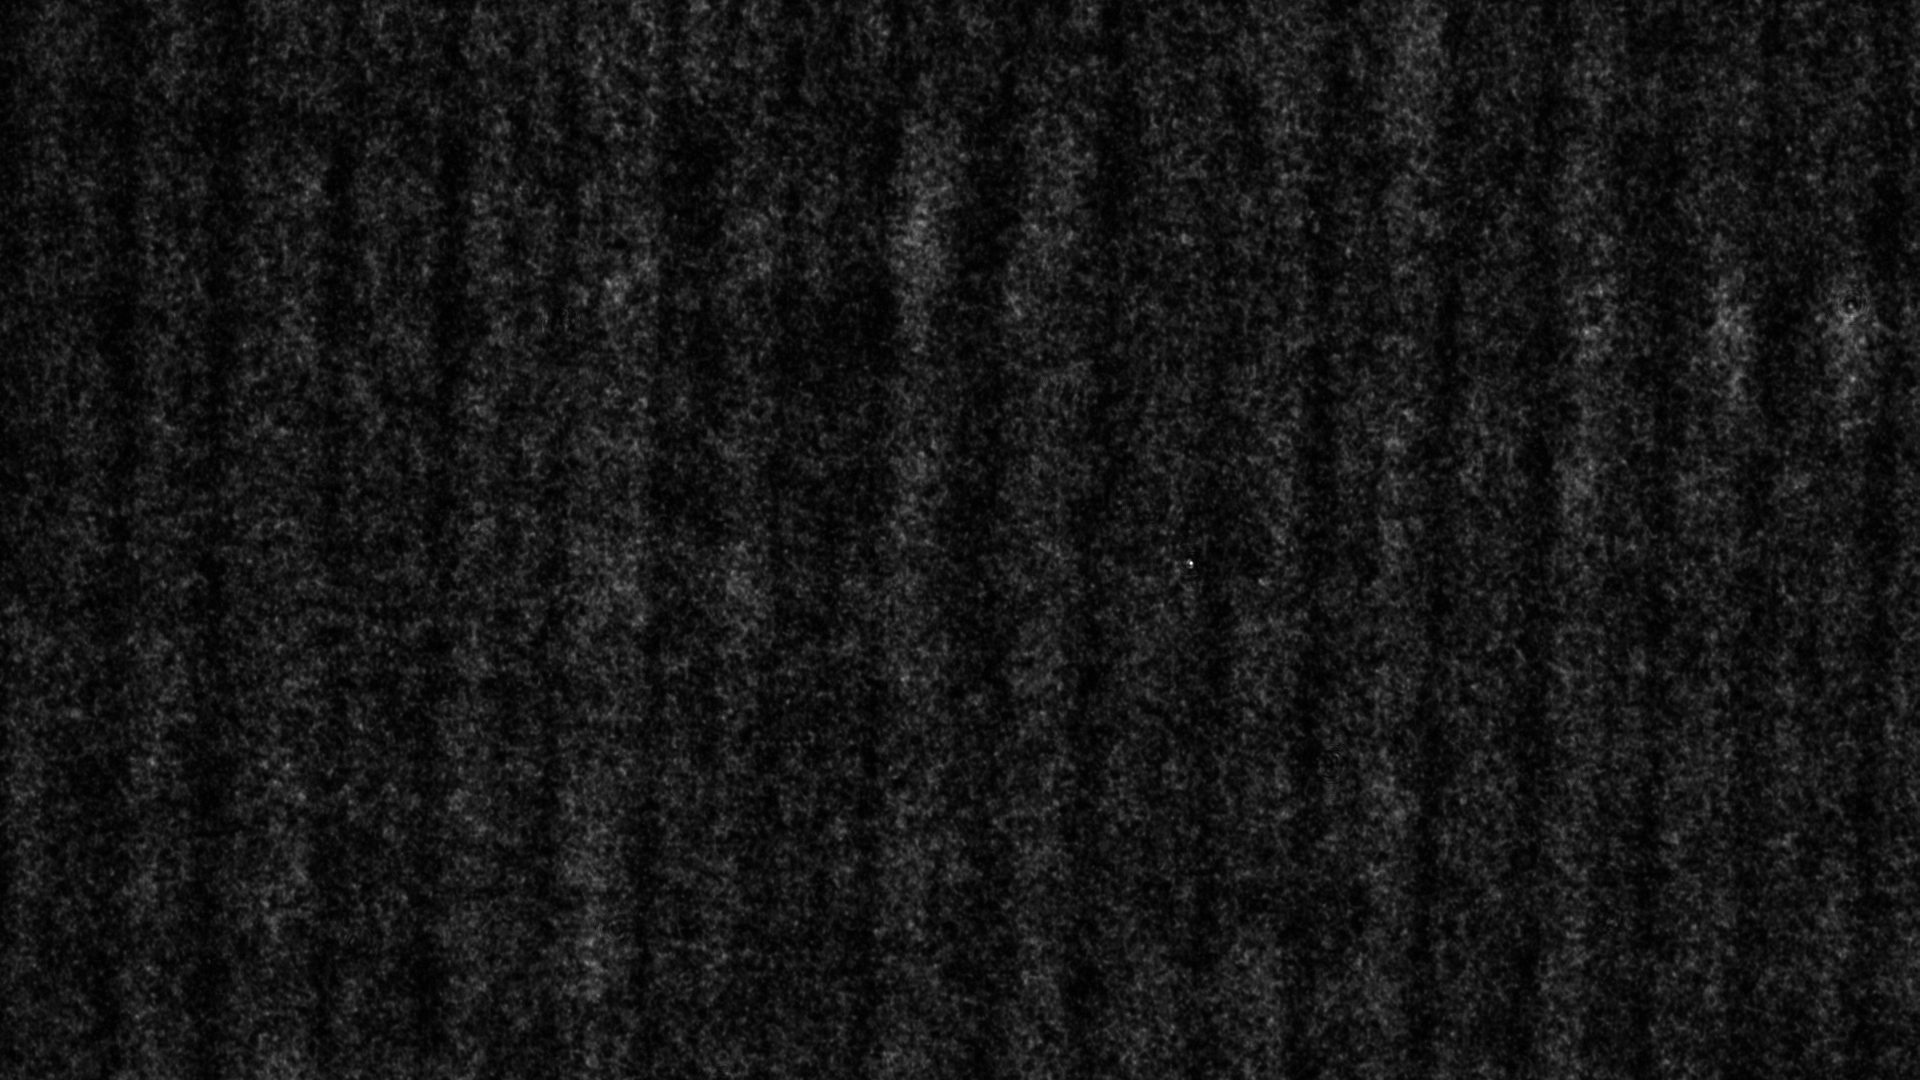
\includegraphics[scale=0.15]{42.2-talbot.png}
    \caption{Imagen del objeto a $18,5 cm$, aproximadamente un cuarto de la distancia de Talbot: $z_T/4$}
    \label{fig:imagen-zt-cuartos}
\end{figure}


\subsection{Periodo de la red}
En nuestro sistema, hemos encontrado que esta distancia vale $Z_T = 72,9 cm$. Conociendo la longitud de onda del láser, $\lambda = 635 nm$, se puede despejar el periodo de la red de la ecuación \ref{ec:zt}, obteniendo:

\begin{center}
    $d = 481,1 \mu m$
\end{center}

\subsection{Cuestiones}
\subsubsection{Cuestión 1}
\subsubsection{Cuestión 2}
\subsubsection{Cuestión 3}





\section{Espectro de Fourier}
\textcolor{blue}{Añadir pequeña introducción}

En esta sección vamos a ver el espectro de Fourier. Para ello montamos el sistema de la figura \ref{fig:montaje-fourier}

\begin{figure}[h!]
    \centering
    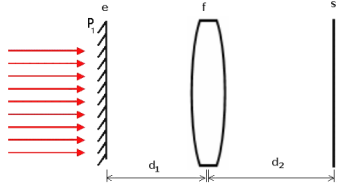
\includegraphics{montaje-TF.png}
    \caption{Montaje experimental para observar el espectro de Fourier}
    \label{fig:montaje-fourier}
\end{figure}

A continuación se muestran los espectros de Fourier que se obtuvieron de diferentes imágenes:

\textcolor{red}{Estaría bien conseguir fotos de los objetos (las diapositivas de las letras y la de los coches) y hacer una figura con varias imagenes en la misma figura, 2x2 por ejemplo.}






\section{Filtrado óptico}




\section{Formación de imágenes con luz parcialmente coherente}









\end{document}